\documentclass[aspectratio=169,10pt]{beamer}
\usetheme{default}
\usecolortheme{dove}
\usepackage{booktabs}
\usepackage{graphicx}
\usepackage{xcolor}
\setbeamertemplate{navigation symbols}{}
\title{DPOE Autoresearch Stress Test}
\subtitle{Closed experiments, bounded claims, proposed plan iteration}
\author{Agent-prepared factual material; critique and reflection reserved for the human}
\date{Lossfunk Autoresearch Challenge}
\begin{document}
\begin{frame}
  \titlepage
\end{frame}

\begin{frame}{Starting research question and claims}
\textbf{Question:} Can calibrated MLLM reward uncertainty improve visual-domain adaptation when the same epistemic signal is used pessimistically and optimistically?
\begin{enumerate}
  \item C1: calibration matters more than reward-model capacity.
  \item C2: epistemic, not aleatoric or matched noise, drives benefit.
  \item C3: coupled reward pessimism (P), adaptive KL (K), and optimistic collection (O) beats either half.
\end{enumerate}
The submitted plan targeted Qwen2.5-VL models, visual manipulation, 5 seeds, and millions of environment steps. The sprint tested only CPU-scale mechanisms.
\end{frame}

\begin{frame}{Autoresearch flow}
\begin{columns}[T]
\column{0.48\textwidth}
\textbf{Driver: OpenAI Codex}
\begin{itemize}
  \item hardware/literature audit
  \item MVE design and implementation
  \item locked execution and analysis
  \item iterated plan, paper, factual deck
\end{itemize}
\column{0.48\textwidth}
\textbf{Reviewer: Claude Code}
\begin{itemize}
  \item independent checkpoint reviews
  \item blocking validity corrections
  \item some manual human-mediated captures after CLI failures
  \item human account; outside the \$50 sprint budget
\end{itemize}
\end{columns}
\vspace{0.5em}
Human authority controlled session time, experiment sign-off, scope changes, manual review delivery, and experiment closure.
\end{frame}

\begin{frame}{How Voila was customized}
The generic exploration workflow was replaced by a fixed-plan stress test:
\begin{itemize}
  \item no new topic selection: the screened DPOE plan was binding;
  \item hardware audit before MVE design; full MLLM plan explicitly out of scope;
  \item 2--3 falsification-oriented MVEs with support/kill criteria;
  \item Claude review and human sign-off before execution;
  \item \texttt{PROGRESS.md}, \texttt{LEARNINGS.md}, and \texttt{BUDGET.md} as resumable audit trails;
  \item negative/null/untested results treated as first-class outputs;
  \item human-only critique and reflection protected from agent drafting.
\end{itemize}
Sessions were time-boxed by the human (3h, 8h, then 4h blocks).
\end{frame}

\begin{frame}{Compute-driven de-scope}
\begin{tabular}{p{0.36\textwidth}p{0.54\textwidth}}
\toprule
Available & Consequence \\
\midrule
4 CPU cores / 8 threads & NumPy-scale synthetic tests \\
5.8 GiB RAM + 4 GiB swap & no local multi-billion-parameter MLLM \\
No accessible NVIDIA GPU & C1 MLLM comparison deferred \\
\$50 ceiling; about \$20 driver inference & local experiments cost \$0 \\
\bottomrule
\end{tabular}
\par\vspace{1em}
MVE 1 never ran. MVE 2 tested the frozen/online uncertainty mechanism; MVE 3 tested coupling validity and solvability.
\end{frame}

\begin{frame}{MVE 2: frozen uncertainty did not acquire information}
\begin{itemize}
  \item 50 locked seeds; three shifts; aligned, decorrelated, and anti-correlated layouts.
  \item Frozen epistemic minus point: +0.0719 aligned, -0.0036 decorrelated, -0.0719 anti.
  \item Visits cannot update a frozen reward model: apparent gain followed static alignment.
  \item Online epistemic beat aleatoric by +0.0081 [0.0030, 0.0131], but the estimator was weak (AUROC 0.532; Spearman 0.162) and generic controls did better.
\end{itemize}
\textbf{Verdict:} the frozen information-gain rationale is structurally killed; the broader strong-online-estimator claim is unresolved.
\end{frame}

\begin{frame}{MVE 2 result landscape}
\centering
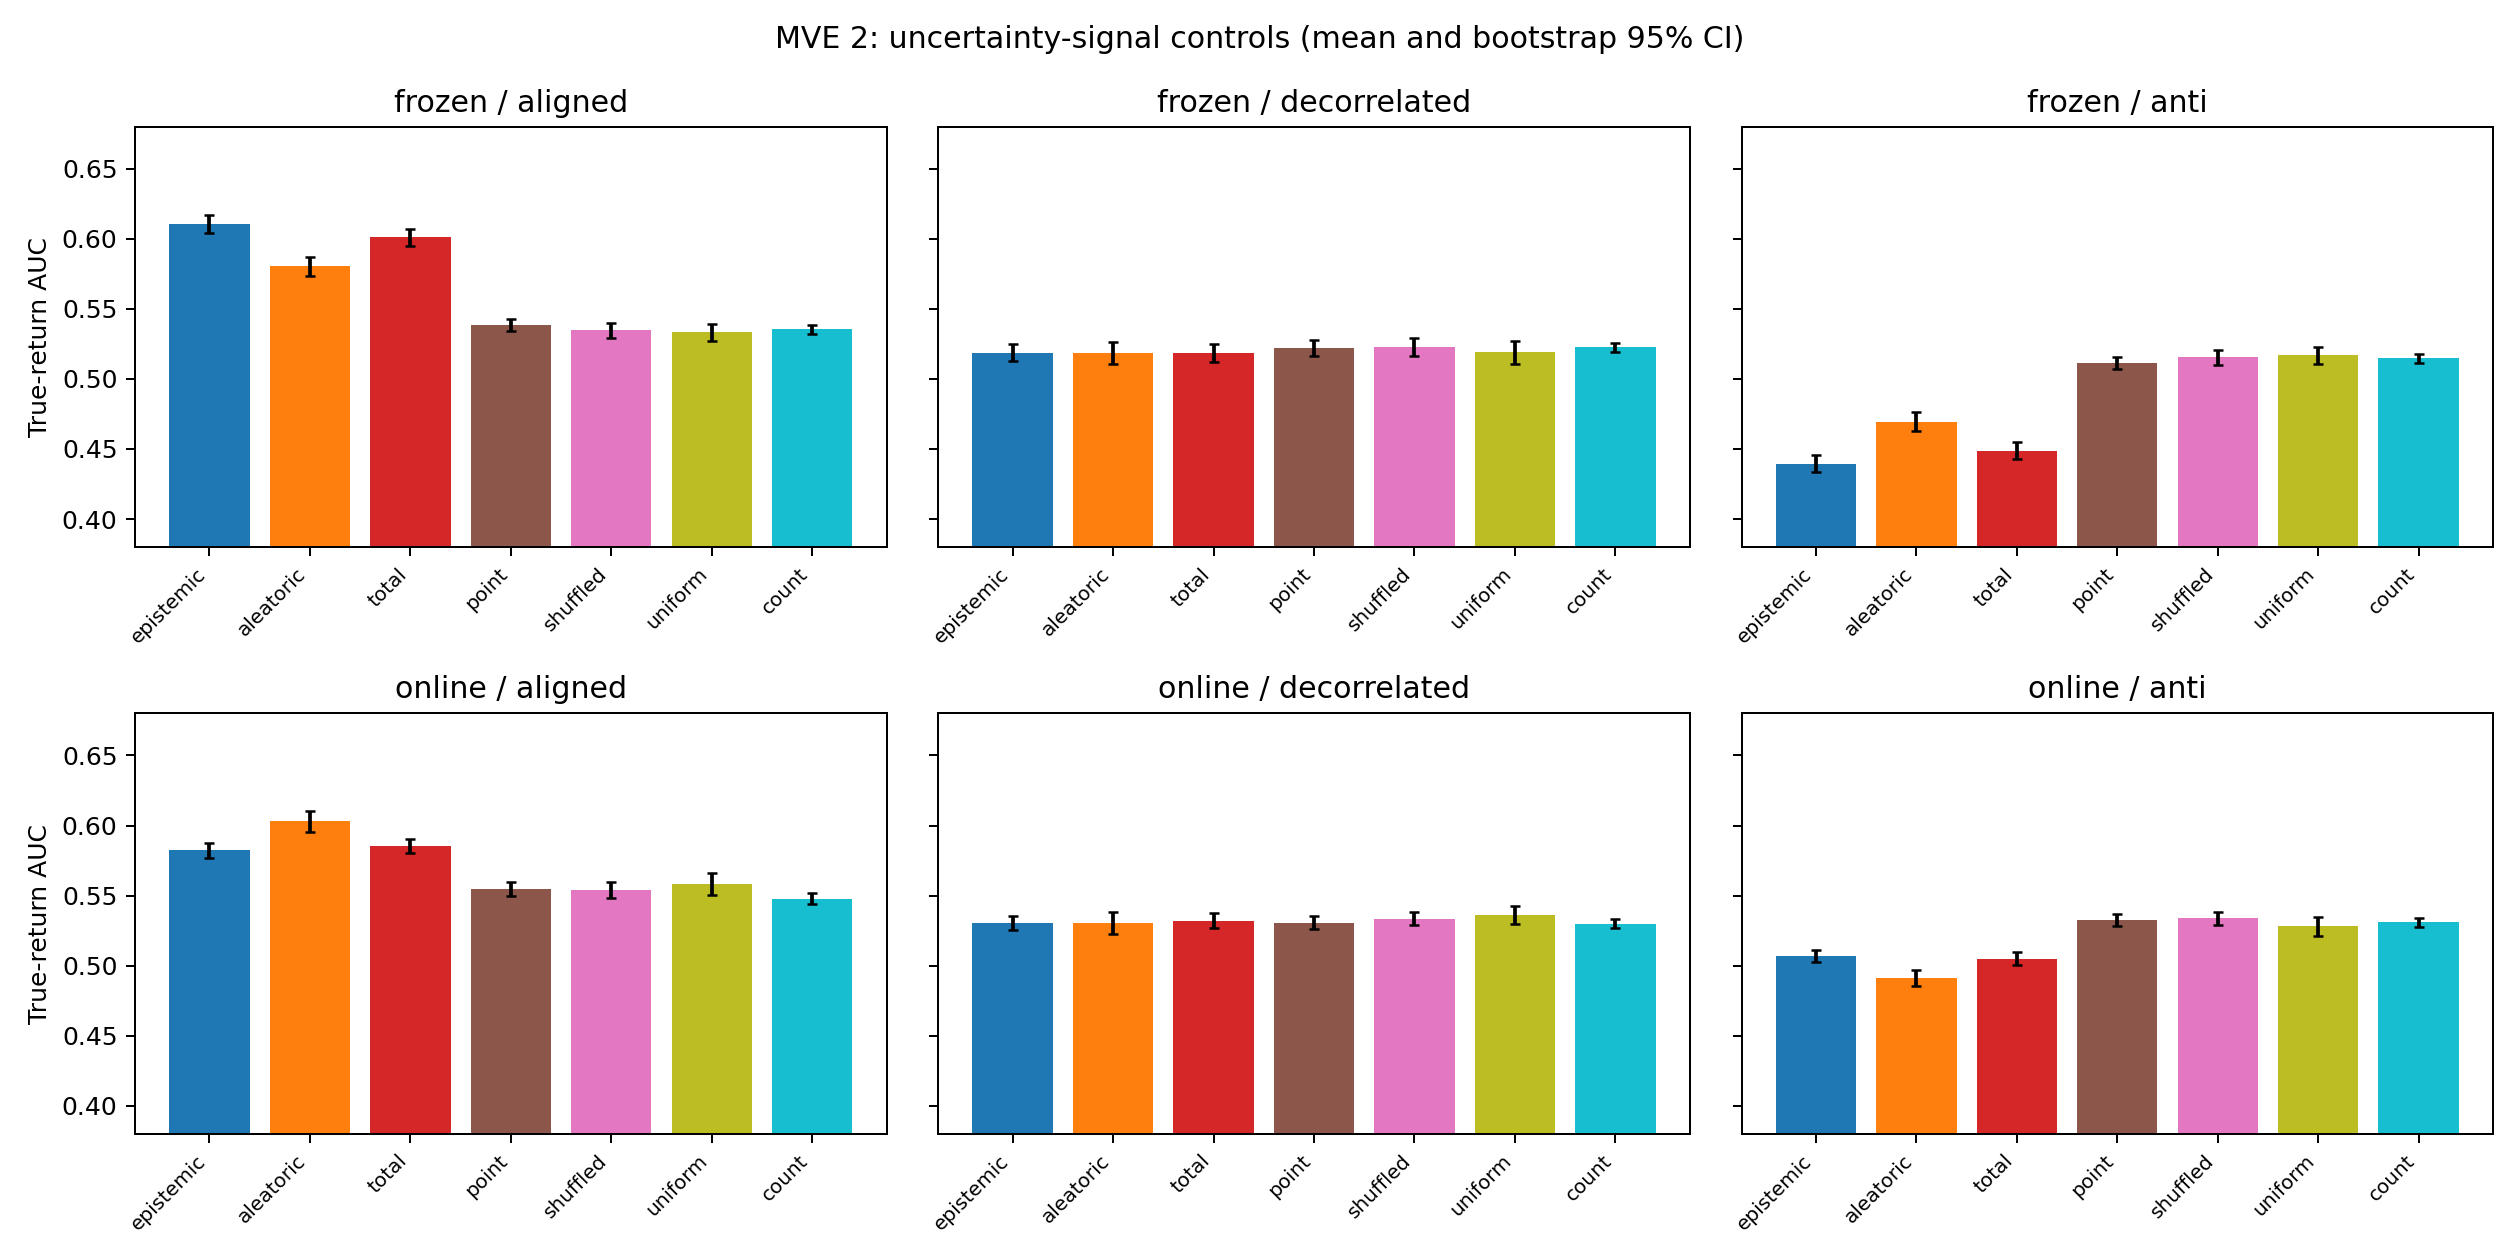
\includegraphics[width=0.88\linewidth]{../results/mve2-full/returns_by_condition.png}
\end{frame}

\begin{frame}{MVE 3 v1: the apparent kill was invalid}
\begin{columns}[T]
\column{0.48\textwidth}
\begin{itemize}
  \item 4,800 locked factorial cells; controlled signal passed quality and leakage gates.
  \item Preregistered rule recorded \emph{killed-at-toy-scale}.
  \item Independent review exposed exploitation true-goal AUC 0.0004 (P+K+O: 0.0002).
  \item Kill withdrawn via disclosed post-review validity amendment.
\end{itemize}
\column{0.50\textwidth}
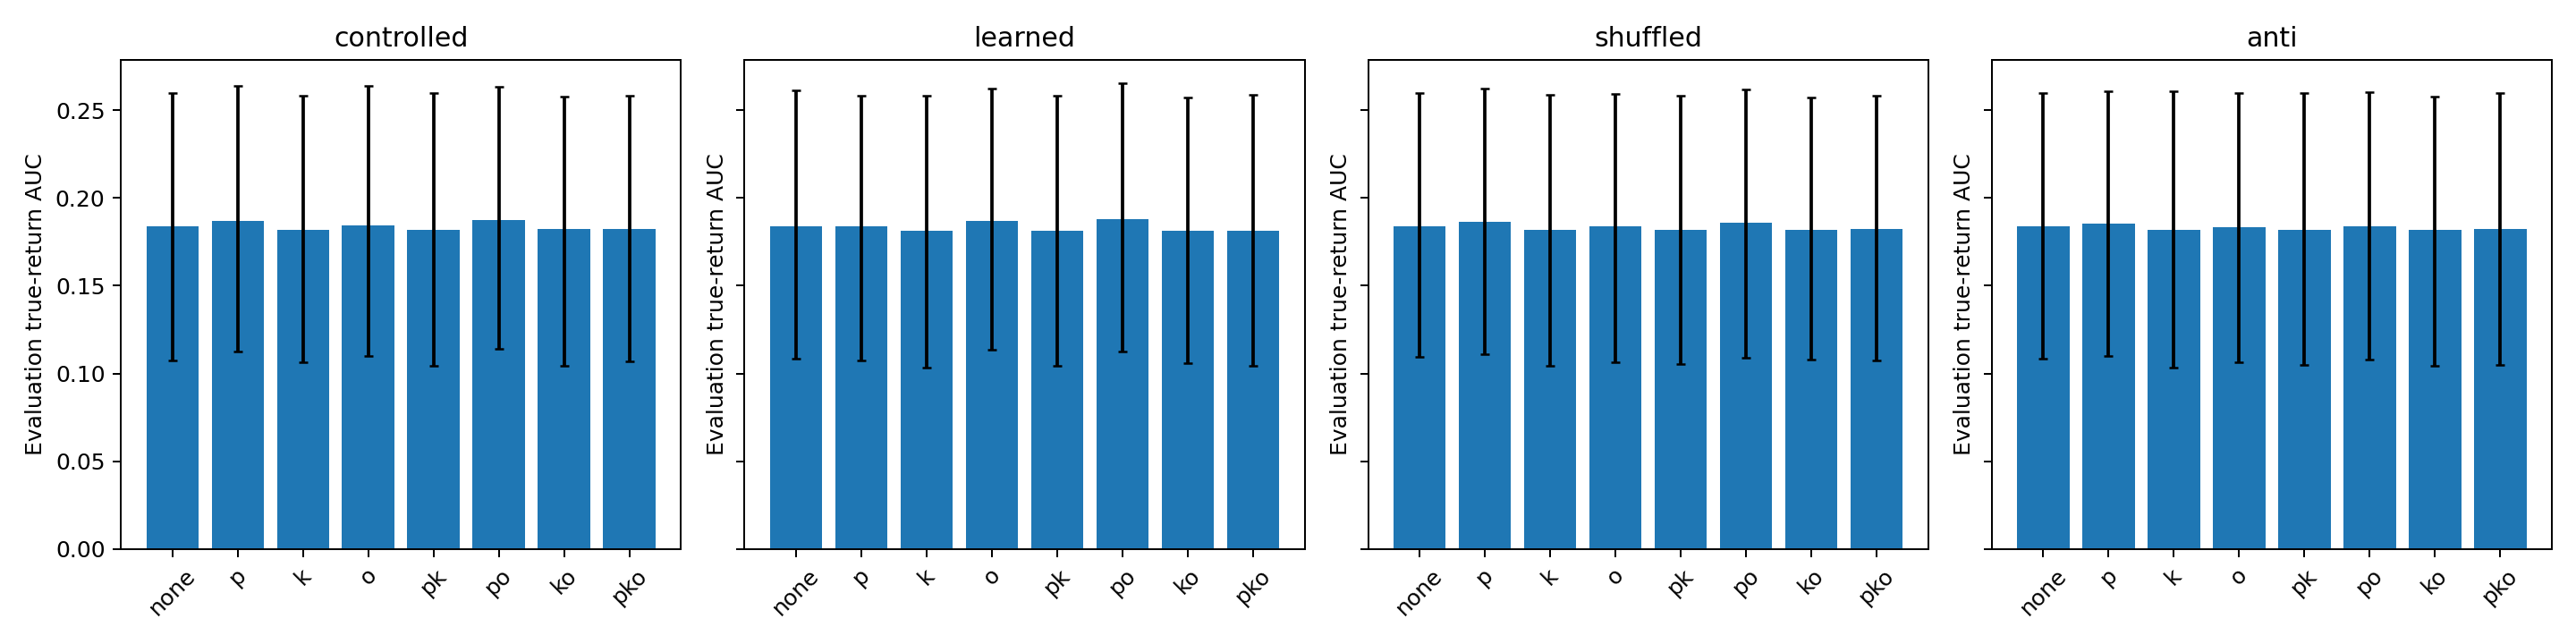
\includegraphics[width=\linewidth]{../results/mve3-locked/return_auc_factorial.png}
\end{columns}
\textbf{Final v1 status:} untested-design-floor-policy-collapse.
\end{frame}

\begin{frame}{MVE 3 v2: bounded solvability failure}
Complete preregistered 27-tuple development grid:
\begin{itemize}
  \item best tuple: $\tau_{ref}=0.18$, $\beta_0=0.10$, clip $\pm1.75$;
  \item oracle goal success 16.44\% vs required 25\%;
  \item oracle-minus-none gap 11.36 pp vs required 15 pp;
  \item return-AUC separation passed at 0.3485;
  \item best tuple was on the relaxation boundary.
\end{itemize}
\textbf{Conclusion: not solvable within the preregistered grid.}

No adaptation-engagement gate, pilot-v2, or locked-v2 seed was opened.
\end{frame}

\begin{frame}{Closed claim table}
\small
\begin{tabular}{p{0.16\linewidth}p{0.76\linewidth}}
\toprule
Claim & Status \\
\midrule
C1 & \textbf{Untested.} MVE 1 did not run; DriveReward forces specialization/data/reward-scale controls in any future test. \\
C2 & \textbf{Frozen information-gain rationale structurally killed analytically and corroborated by MVE 2.} Online claim unresolved. \\
C3 & \textbf{Untested at toy scale.} v1 exploitation floor; v2 not solvable within the preregistered grid. \\
\bottomrule
\end{tabular}
\end{frame}

\begin{frame}{Proposed research-plan delta}
\begin{enumerate}
  \item Separate frozen-RM risk control from online-RM active learning.
  \item Gate estimator claims on shifted error prediction and calibration.
  \item Require oracle reachability, return headroom, and factor-independent adaptation engagement before a coupling factorial.
  \item Use a complete $P\times K\times O$ factorial with practical effect floors and explicit hacking denominators.
  \item Reframe C1 around calibration \emph{after} controlling specialization, data, reward scale, calibrated-large, and matched compute.
\end{enumerate}
This is an agent-proposed revision; the human decides the final delta.
\end{frame}

\begin{frame}{HUMAN-ONLY: Merciless critique of the AI artifact}
\centering
\Large \textbf{PLACEHOLDER --- HUMAN AUTHOR ONLY}

\vspace{1.5em}
\normalsize The agent intentionally supplied no critique content on this slide.
\end{frame}

\begin{frame}{HUMAN-ONLY: Reflection on autoresearch limits}
\centering
\Large \textbf{PLACEHOLDER --- HUMAN AUTHOR ONLY}

\vspace{1.5em}
\normalsize The agent intentionally supplied no reflection content on this slide.
\end{frame}

\appendix
\begin{frame}{Appendix: exact prompts and user decisions}
\scriptsize
\textbf{Reviewer invocation pattern:}\\
\texttt{claude -p "REVIEW REQUEST: <what you did and why>. Files to review: <paths>."}

\vspace{0.5em}
\textbf{Human decisions retained verbatim:}
\begin{itemize}
  \item \textit{Approved, start MVE 2 now, log the sign-off.}
  \item \textit{Final sign-off: implement and execute MVE 3 exactly under the approved protocol. Ensure the locked run can resume from the last completed cell after an interruption rather than restarting. Log this as a user decision.}
  \item \textit{Experiments are closed. MVE 1 will not run.}
\end{itemize}
The full session narrative and additional decisions are in \texttt{PROGRESS.md}.
\end{frame}

\begin{frame}{Appendix: reviewer trail highlights}
\small
\begin{itemize}
  \item Reviews 01--07: MVE protocols revised to approval before locked execution.
  \item Review 08: exposed v1 exploitation floor; prevented an invalid C3 kill.
  \item Reviews 09--14: forced deviation disclosure, solvability gates, audit repair, and report-only regeneration.
  \item Review 15 was REVISE, not the initially reported APPROVE; stale v1 pilot naming fixed.
  \item Review 16: restored related work, reviewer provenance, missing deviations, accurate title, and compilable paper.
  \item Review 17: corrected the inherited Zhang/AdvPO citation to the stored Kang--Oh ICLR 2025 paper.
\end{itemize}
Some later reviews were human-mediated manual Claude runs after empty/API-error CLI captures.
\end{frame}

\begin{frame}{Appendix: time and cost actuals}
\small
\begin{tabular}{p{0.29\textwidth}p{0.35\textwidth}p{0.19\textwidth}}
\toprule
Work & Actual & Dollar cost \\
\midrule
MVE 2 locked run & 257.7 s & \$0 \\
MVE 3 v1 locked run & 8,462.3 s (2.35 h) & \$0 \\
MVE 3 v2 report-only audit & same development namespace & \$0 \\
Driver inference & session-spanning & about \$20 \\
\bottomrule
\end{tabular}
\par\vspace{1em}
Claude review used the human's personal account and was outside the \$50 sprint budget.
\end{frame}

\begin{frame}{Appendix: artifact map}
\small
\begin{itemize}
  \item Paper: \texttt{paper/dpoe\_negative\_result.pdf}
  \item Proposed plan: \texttt{iterated-research-plan.md}
  \item MVE 2: \texttt{mve2/}, \texttt{results/mve2-full/}
  \item MVE 3 v1: \texttt{mve3/}, \texttt{results/mve3-locked/}
  \item MVE 3 v2 gate: \texttt{mve3v2/}, \texttt{results/mve3v2-development/}
  \item Audit trail: \texttt{PROGRESS.md}, \texttt{LEARNINGS.md}, \texttt{BUDGET.md}, \texttt{reviews/}
\end{itemize}
\end{frame}
\end{document}
